\chapter{Instrument Suite}

* Total mass and power requirement

* What do we want to measure and why? Explain why some instruments were picked and some were discarded (we can use the notes from when we did that in class)


\autsection{Sample up-concentration \& injection}{Morten Lykke Hilligsøe}

Although the instruments selected for the mission have high detection rates, up-concentration of the surrounding waters will enable the detection and quantification of low concentration compounds. To do this, the surrounding water is passed through a ceramic nano filter, which retains any microbes such as bacteria and viruses, as well as most particles. The filter was originally developed in collaboration with NASA, for use in water recycling systems on space missions. After running the surrounding water through this filter for an extended period of time, the water flow is reversed and directed to the instrument suite. When reversing the water flow, the particles on the surface of the filter will be extracted relatively quickly, thereby resulting in an up concentrated sample liquid.

In order to reverse the water flow, a pump is needed. Peristaltic pumps are mechanically very simple and reliable, and therefore suitable for space missions. However the HPLC system described in section \ref{sec:hplc}, requires a pump operating at pressures outside the range of most peristaltic pumps. In order to combine the two pumps of the filtration system and HPLC system, a single high pressure pump \cite{} is used. The suggested high pressure pump has a maximum flow rate of 40ml/min at 500 psi, and most likely higher at lower pressures. 40ml/min isn't a lot, but it accumulates to 57,6l of water per day. If 50l of water is filtered in 1 day, and the filter residue can then be extracted into 50ml of sample water, an up-concentration factor of 1000 has been achieved, which should be sufficient for most experiments.

To direct the water flow several valves will also be required. Figure \ref{fig:filter} presents a water filtration system, complete with valves and tubing, which can be implemented inside the penetrator, allowing up-concentration of the surrounding water. In this system, a disk-shaped filter is used in combination with a central valve which open or blocks the water flow into the instrument suite, as well as a system of valves (flaps) which opens or blocks external water flow to up-concentrating side of the filter. After the sample reaches the instrument suite, other valves can direct which specific instruments should receive the sample.

\section{Sample handling}

* We need a design, I (Kristian) talked with some other about this, but we need to coordinate with the rest of the groups
   (SMS http://www.esmats.eu/amspapers/pastpapers/pdfs/2008/mumm.pdf)

* Sample rate

* What is under pressure and what is not?

* Order of the instruments

\subsection{Robot Arm} % Rasmus


\section{CTD/ADCP}

* Includes temperature probe

    * We will properly need more around the body of the penetrator

\section{Light sensor}

\autsection{Gas detector}{Agge Winther}

This chapter concentrates on why gas detection is important when searching for life, and how an instrument is designed for use in the penetrator to detect different gasses.

First a look into what gasses to be expected on Europa, next a look into gas detection under normal circumstances, and lastly a design of a gas detector for specific use in the ocean of Europa.

\subsection{Theory}

The main objective for this mission is to search for life. As explained in earlier chapters this could be found in many shapes and sizes. From bacteria to small living organisms, or perhaps alien life forms, unknown to science. If Europa is a life harbouring planet, and the ocean under the ice contains some sort of life. Then it would be an idea to also investigate extinct life.

Assuming the type of life can be compared to that of earth, we should be able to detect bi-products from living organisms. This chapter focuses on gasses, produced by living organisms, decomposed organic material or nutrients to support life.

As know from life and living organisms on earth, most life depend on the sun to create some sort of photosynthesis. Under the ice of Europa little to no light is expected to be found due to the thickness of the ice sheet above. Therefore traditional life, driven by the sun, is not to be found in the water of Europa, but for life harbouring conditions, some energy must be available.

Look back at earth, only a few places exist where life thrives, without light. One of them is around the black smokers on the ocean floor. The reason for mentioning this example is that Europa studies\cite{schmidtocean} show that a source of energy could be similar to the black smokers on earth. Life is found in great abundance around the smokers. First it was thought the organisms lived on marine snow, but the amount of life compared to the little amount of marine snow, would not be able to sustain the large amount of organisms found. Now it is know that the organisms thrive on the bacteria living around the smokers. This is called chemosynthetic bacteria, and instead of using photosynthesis the bacteria uses the nutrients and hydrothermal fluids from the smokers. The bacteria uses sulfur, methane and heat the create the energy need for life, this then feeds other life like clams and tubeworms, and usually a small ecosystem is found around black smokers, even if there is now sunlight. Some of the organisms around the smokers do depend on oxygen but anaerobic organisms are also found\cite{PMEL}.

This is good indication for life and even if the smokers are long gone, decomposition of the bacteria and ecosystems around the smokers could be seen in the levels of sulfur, methane, ethane, $CO_2$ and other hydrocarbons found in the water. Therefore sensors which can detect hydrocarbons would be ideal to bring with the penetrator down to the ocean, and look for these gasses.

\subsubsection{Searching for hydrocarbons}

Hydrocarbons are organic compounds made from carbon and hydrogen. Overall hydrocarbons can be dived in the 4 groups:
\begin{itemize}
  \item Saturated hydrocarbons (alkanes)
  \item Unsaturated hydrocarbons (alkenes)
  \item Cycloalkanes
  \item Aromatic Saturated hydrocarbons
\end{itemize}
Where methane and ethane is alkane's due to their single bond. On Earth most hydrocarbons come from decomposed organic matter, and it is this connection that will help conclude the kind of life on Europa.

Taking into account the smokers, organic material and simple life forms, simple hydrocarbons and other gasses would be found dissolve in the water or as gas bubbles. From this point on the focus shift towards detecting these gasses, which include: $SO_2$, H2S, $CH_4$, $NH_3$, $CO_2$, C2H6. The sensor need to be design must be able to detect as many as possible and if feasible, even bigger alkenes, alkanes and aromatic compounds.

\subsubsection{Detecting hydrocarbons at low pressure}

Detecting hydrocarbons can be done in many ways, first a look into how detection of gasses is done on Earth. This will give an idea on how today's methods could be modified and implemented in the instrument suite on the penetrator.

Most gas detectors are used to detect gasses harmful to humans, and leaks in pipelines. Most detectors are used to detect gasses in industry for safety reasons, helping to detect toxic, flammables or oxygen depletion, dangerous to workers or work safety. The most common ways to detect gas are:
\begin{itemize}
  \item Electrochemical
  \item Infrared
  \item Semiconductor sensor
  \item Ultrasonic
  \item Holographic
\end{itemize}
Electrochemical gas detectors diffuses the gas through a membrane, into an electrode, where it is oxidized. The reaction between the electrode and the gas generates an electric current which is linear to the gas concentration and by changing the membrane it is possible to custom design a detector for a specific gas. This type of sensor is very simple, stable and robust, but it is not perfect, it suffers from cross sensitivity and if it gets in contact with corrosive compounds, its life of operation is shortened\cite{intlsensor}.

Infrared gas detecting uses a whole other method to determining the gas in question. Here infrared light is passed through a known volume of gas, and the absorption of the different wavelength in the infrared spectrum is then analyzed. Different gasses have different absorption spectrums, like a fingerprint, and thereby the gas can be determined. This technique is more complex, but a lot more flexible compared to the electrochemical sensor, since it is able to detect different gasses with the same detector\cite{ndir}.

Semiconductor sensors detect gas by a chemical reaction with the semiconductor material, most used is tin-oxide, as gas comes in contact with the tin-oxide the resistance through the material drops. This type of sensor is commonly used for detection of methane, carbon monoxide, hydrogen, oxygen and alcohol-vapor.

Ultrasonic gas detectors are mostly used for detecting leaks, and cannot determine gas concentration. It works by listing for changes in the background noise around ultrasonic frequencies, since high pressure gas-leaks emit ultrasonic sounds, which can be detected. It is therefore no good for the type of detection wanted for this mission.

Lastly there are holographic gas sensors; they work under much the same principle as for the infrared detectors. Here the change in the reflected wavelength from the hologram can be used to determine the composition of the gas in front of the hologram. To work, they do require white light or lasers, which makes them more complex then the infrared sensors.

All of these methods mention above can be used on a gas, but a gas is just a state of the specific compound in question. On earth the gasses mentioned previously ($SO_2$, H2S, $CH_4$, $NH_3$, $CO_2$, C2H6) are naturally occurring as gas at sea level, (1 atm, 20 C), but this is not the case at the crushing pressure under the ice.

\subsubsection{Gas detection at Europas ice-sea surface}

The exact composition of Europas internal geology is still unknown. Qualified guess can be made dependant on pictures and its orbit. From this, it is estimated that the ice could be proximately 10km thick, all this ice generate an enormous pressure, estimated to be between 100-200bars at the ice-water barrier. Therefore what on Earth is a gas, would be a liquid or supercritical where the penetrator is sitting analyzing samples. To get a better insight into what happens to a compound mixed with water under this pressure a small study is done below.

At the ice-water barrier the temperature is around 273.15 Kelvin, below this the water starts to freeze and above it melts at a pressure of 100 bar\cite{PhaseH20}. At 200bar the temperature will be a 3 to 5 degrees Kelvin lower due to the pressure, but in general the freezing temperature is constant\footnote{This is for pure $H_2 O$}.

Overall a substance can have 3 states, gas, liquid or solid, it can also become super critical where it is in-between all 3 states. The way to characterize the states of a substance is through its phase diagram. An example of this is $CO_2$, which have the following phase diagram.

\begin{figure}[htb]
  \centering
  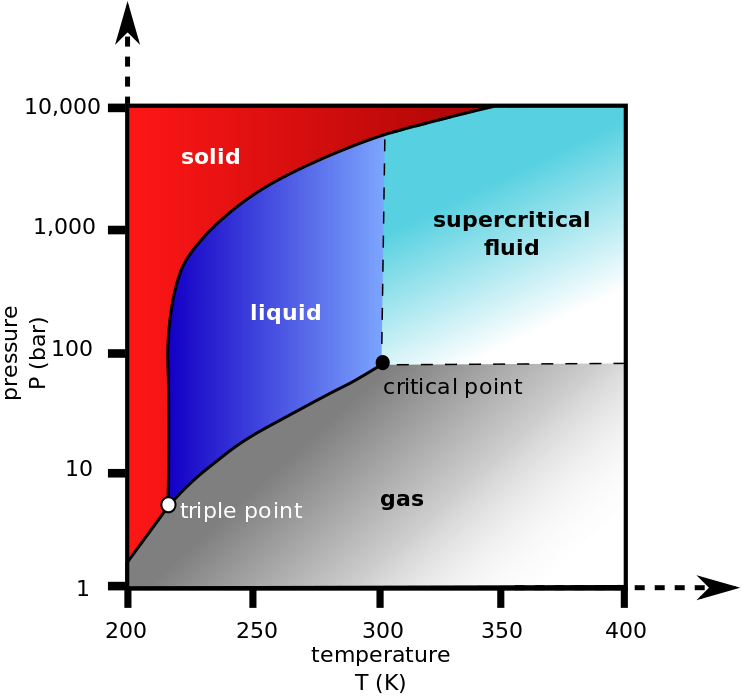
\includegraphics[scale=0.4]{figures/GasDetectionAgge/CO2PhaseDiagram}
  \caption{Phase diagram of $CO_2$, here the different phases are clearly seen, and how they depend on pressure and temperature\cite{PhaseCO2}}
  \label{fig:PhaseDiagramCO2}
\end{figure}

In the phase diagram of $CO_2$ (\ref{fig:PhaseDiagramCO2})it can be seen how the phases depend on pressure and temperature. If there is $CO_2$ present in the water at Europa, it would not be as a gas, because at 100 bar and 273.15 Kelvin $CO_2$ is liquid.

If $CO_2$ is present in the water, it is most likely to be mixed in the water, since water is a very good solvent for ionic and organic compounds, which makes most substances soluble in water; this is also the case for the gasses in question here. The solubility of substance in the water depends on the pressure above the solution. This follows Henry's law which states that the "solubility if a gas in liquid is directly proportional to the pressure above the surface of the solution\cite{SolubilityOfGases}".

This can be demonstrated with a bottle of soda. When the bottle is opened the pressure is released and CO2 starts to bubble up because the water cannot contain the same amount of $CO_2$ in the soda, under 1atm pressure.
As the phase diagram, a graph of the solubility of a substance can be made; here it is the solubility of $CO_2$ in water, but at atmospheric pressure:

\begin{figure}[htb]
  \centering
  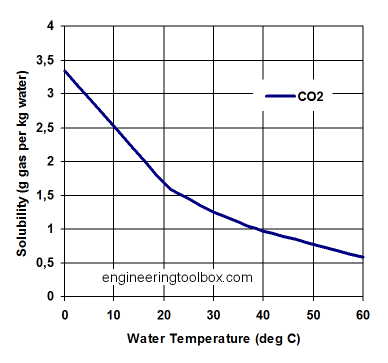
\includegraphics[scale=0.4]{figures/GasDetectionAgge/CO2Solubility}
  \caption{The solubility of $CO_2$ gas in water, at atmospheric pressure\cite{SolubilityOfGasesInWater}}
  \label{fig:SolubilityofCO2}
\end{figure}

From \ref{fig:SolubilityofCO2} it is seen that approximately 3.4 grams of $CO_2$ gas can solute in water at 273.15 Kelvin at a pressure of 1 atm. Combining this with Henry's law, the amount increases proportionally with the pressure, so the amount of $CO_2$ the water is able to solute is grater at 100 bar. Even when the $CO_2$ is liquid the solubility can be approximated as a gas/liquid solution\cite{SolubilityExplained}.

The conclusion on this is, it is not possible to use "normal" gas detecting methods, as discussed above. Other methods are needed to be able to detect what substances are present in the water. Some of the substances like $CO_2$ and $SO_2$ will be a liquid mixed with water, others might be a gas or super critical. The way of detecting the substances in the water needs to be done on another way.

\subsection{Implementation}

From the theory section it was discussed how to detect gasses, and what problems, and complications this have at high pressure, between the water and ice at Europa. The main problem in gas detection at Europa, concerned the fact that most of the gasses are liquid and not a gas. Therefore an instrument is design to take advantage of this high pressure condition. First the substances of interest are indexed according to their phase, solubility and at what pressure they change phase from liquid to gas (at constant temperature of 273.15 K) under the ice. Here the assumption is 100 bar and 273.15 degrees Kelvin.

\begin{table}
  \resizebox{\textwidth}{!}{%
  \begin{tabular}{|c | c | c | c|}
    \hline
     Substance: & Solubility: (g/kg water) & State: & Phase change pressure\cite{GasEncyclopedia} [Bar] \\ [0.5ex]
    \hline
    $SO_2$ (Sulfur dioxide) & 225 & Liquid & 1.5\\
    \hline
    $CO_2$ (carbon dioxide) & 3.4 & Liquid & 35\\
    \hline
    $NH_3$ (Ammonia) & 900 & Liquid & 4\\
    \hline
    $H_2 S$ (Hydrogen sulfide) & 7 & Liquid & 6\\
    \hline
    $C2H6$ (Ethane) & 0.13 & Liquid & 25\\
    \hline
    $CH_4$ (Methane) & 0.04 & Gas/Super & NA\\
    \hline
  \end{tabular}}
\end{table}

As mention in the Theory section, these substances are of great interest to detect possible life/extinct life in the water, for now on the focus will be on these 6 compounds for the further development of an instrument for the penetrator.

From the table above it is noted that all of the compounds are soluble in water, and most of them as a liquid at 100 bar and above. The notable characteristic is the phase change pressure, where the liquid changes phase to a gas. The important thing here is different pressures where the phase change happens, as for the IR-gas detector, this is a fingerprint tied to the compound. The odd one out is methane, it is still in a gas or supercritical state; it could therefore be detected with standard methods already known.  This will be investigated later.

The idea is to use an expansion chamber to boil of the gasses by lowering the pressure slowly. In constant temperature conditions a slow expansion of the gas, will give a characteristic pressure graph, with flat spots as the compound boils off and changes it phase. The principle can be seen in \ref{fig:PVdiagram} below.

\begin{figure}[htb]
  \centering
  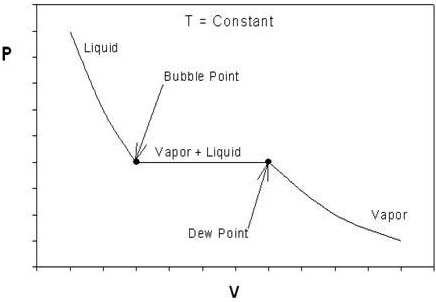
\includegraphics[scale=1]{figures/GasDetectionAgge/PVdiagram}
  \caption{PV-diagram with constant temperature. As the volume expands, the pressure drops, and the liquid changes state into gas}
  \label{fig:PVdiagram}
\end{figure}

In the PV-diagram, going from left to right, the liquid follows an isotherm as the pressure drops, when it reaches it phase change, and the liquid boils of into a gas. As this happens the pressure remains constant. With the help of a pressure sensor this can be detected, and the gas identified.

To create this phase change the pressure of the liquid under test needs to be dropped. If an expansion chamber is used then the Europa's liquid water will enter at a 100 bar or above, and then the pressure needs to be slowly drop down to 1 bar to detect compounds such as sulfur dioxide.

A traditional expansion chamber consists of a chamber with a moving piston that increase the volume in the chamber and thereby the pressure. This is not optimal for space exploration; firstly the need for moving parts is a source of unreliability and problems. Next to move the piston, a vacuum pump would be need. This also contains moving parts and is fragile, due to high pressure differences and high pressure seals, this method are therefore not ideal at all for the penetrator.

If it is not possible to create a low pressure by means on-board the penetrator, it needs to be brought from Earth, in small vacuum cylinders. This is a more reliable method but it life cycle is fixed to the number of cylinders brought with the penetrator.

\subsubsection{Detection chamber}

This method will consists of one chamber with the liquid sample under testing, and a vacuum cylinder connected through a small sealed hole into the test chamber. When the test chamber is ready for test the seal is punctured letting the pressure inside the test chamber slowly decrease, while the pressure is closely monitored. The pressure graph will then show the phase change of the compounds contained in the liquid under test. This method also shows other compounds than the 6 specified in the table above, this way if the predictions on what is contained in the water are wrong, the pressure graph will show it and it can afterwards be analyzed back on Earth. This is the design that will be used on the penetrator, the only down side to the instrument is it limited use, due to the vacuum cylinders. Take into account its simplicity, and that the water sample only takes place a few times due to the locked position of the penetrator, this is a good compromise.

\subsubsection{The mechanical design}

This subsection describes the overall mechanical design, including drawings and full description of functionality. First an overview of the complete system is presented:
\begin{itemize}
  \item Vacuum cylinder
  \item Test chamber
  \item Fill and empty mechanism
  \item Cylinder puncture
\end{itemize}
These are the 4 overall subcomponents and functions of the Vacuum Expansion Gas Analyzer (VEGA).

The vacuum cylinder, is based on the small canister, know from siphon bottle. In a siphon it is filled with $NO_2$ but could also contain a vacuum, in \ref{fig:Sipon} a picture of the cylinder is presented.

\begin{figure}[htb]
  \centering
  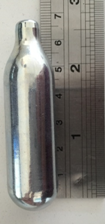
\includegraphics[scale=1]{figures/GasDetectionAgge/SiphonCylinder}
  \caption{A small gas cylinder from a Siphon. Instead gas, it would contain a vacuum}
  \label{fig:Sipon}
\end{figure}

A cylinder of this size has a volume of approximately 13 $cm^3$. This should be enough to let the gasses expand, since most of the liquid water on Europa is expected to be $H_2$O\footnote{\url{http://www.nasa.gov/topics/solarsystem/features/europa20130305.html}, 2016-05-07}, and therefore only a fraction of this is liquid gas. At the top of the cylinder, where it tapers in, the gas is released when punctured. This could be mechanized by a spring, loading the cylinder with nylon string and then burn the nylon string with a small electrode (copper wire) releasing the cylinder into a firing pin, with a small hole in to the test chamber slowly letting the liquid gasses expand.

The liquid under test is contained in the expansion/test chamber, where the vacuum cylinder is connected through the hollow firing pin. The chamber size compared to the vacuum cylinder is the most important ratio, since it determines how low the pressure in the test chamber becomes. The major fact is, as mention, how much liquid "gas" is contained in the water, in the theory section solubility was discussed, but here it was for a gaseousness substance mixed with water and not a liquid gas, further more the pressure is now much higher and Henry's law also needs to be taking into consideration. This part needs further investigation, but for now a good estimate of how much gas that would be in a water sample is 1 \%, this means that 99 \% of the sample is uncompressible. A chamber with a volume of 5 $cm^3$ would contain 0.05 $cm^3$ of liquid gas at 100 bar. To bring this down to 1 bar the volume needs to expand to 5 cm3, more than enough for a vacuum cylinder with a volume of 13 $cm^3$. This gives a satisfying pressure margin of more than 100 \%. Meaning that even with a pressure below the ice of 200 bar the chamber would still be able to reduce the pressure to less than 1 bar. Or if the liquid gas contained in the water is 2 \% of the total volume.

The test chamber needs to be filled and emptied after every use, with inlet and outlet ports in both ends of the chamber. Connected to the inlet and outlet will be a separate solenoid valve, and the pumping system from the other instruments will be utilized to circulate a water sample into the test chamber. The valve system will work by opening the inlet solenoid letting the water fill the chamber, then the valve closes, and the vacuum cylinder is released from its spring mechanism, slowly increasing the volume while the pressure is monitored. The chamber is now at around 1 bar pressure and the outlet valves opens equalizing the pressure, the inlet valve then opens and the chamber is flushed clean. It is very important to thoroughly flush the chamber to avoid any contaminants from previous samples, therefore it is suggested to let the inlet and outlet valve stay open and continually circulate the water surrounding the penetrator, through the chamber. This is of cause only if the sample is taken from the same place all the time, if the penetrator is able to pick up samples from other places then its surroundings a more complex flushing system needs to be implemented.

Lastly the puncture of the cylinder needs to be addressed, as already mention a spring loaded firing pin mechanism, would be the simplest way of implementing the vacuum puncture. This way no motors or valves would be needed, and therefore less points of failure. One of the main problems with this design is to close off the cylinder after the expansion has happened, to avoid that the test chamber volume increase. A way of avoiding this would be the use a two stage spring system, the first stage is fired and punctures the cylinder, when the expansion is done, the next spring fires and blocks the hole with the end of the firing pin.

\begin{figure}[htb]
  \centering
  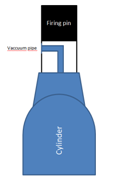
\includegraphics[scale=1]{figures/GasDetectionAgge/Firingpin}
  \caption{The black box is the firing pin where the first part contains the hollow part, which lets the expansion happen, and the solid black is the part that blocks the cylinder after use}
  \label{fig:FiringPin}
\end{figure}

In \ref{fig:FiringPin} an example of such a firing pin is sketched, the box with the black boarder is the firing pin, where the bottom part contains the hollow part, and the top part contains the seal of the cylinder after use. The first stage spring releases and punctures the cylinder, by sending the firing pin down to where the vacuum pipe exits, when the pressure is dropped the next spring releases sealing the cylinder.

The above 4 subsections explains the main parts of the VEGA-instrument, how it works and functions. From this, a hand drawing was made to show how it could look, and to get an idea of the overall dimensions and weight estimate. This first design was made to contain 6 cylinders in a rack structure:

\begin{figure}[htb]
  \centering
  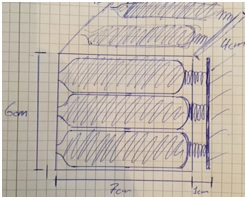
\includegraphics[scale=1]{figures/GasDetectionAgge/CylinderRack}
  \caption{A rack of 6 cylinders, with the spring in the back. Approximate dimensions are 6x8x4cm}
  \label{fig:RackOfSix}
\end{figure}

On \ref{fig:RackOfSix} a sketch of the structure for the cylinders can be seen, in the back the spring system is contained. This rack then connects to the chamber:

\begin{figure}[htb]
  \centering
  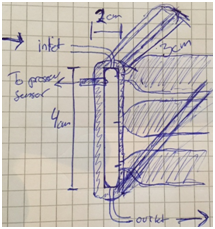
\includegraphics[scale=1]{figures/GasDetectionAgge/ChamberAndRack.png}
  \caption{Cross-section of the chamber and part of the vacuum cylinders, this chamber is 6 $cm^3$ and therefore a little bit too big}
  \label{fig:CrossSectionProto}
\end{figure}

In \ref{fig:CrossSectionProto} a cross section of the chamber is sketched, with part of the cylinder rack. As describe the liquid under test enter through the top inlet and exits at the bottom outlet (the valves are left out). Into the test chamber a pressure sensor is mounted to monitor the expansion. The firing pin is carved into the wall of the chamber and is not visible in the drawing, but when the cylinder is used, the spring will push the cylinder all the way into the wall of the chamber sealing it with the top of the firing pin.

\subsubsection{Principle prototype}

From the drawings and sketches a small prototype was made, which give an idea of how it would look if build. The prototype serves no practical function, and the firing pin or spring system is not build, this is just a chamber with in- and outlet and one cylinder attached.

\begin{figure}[htb]
  \centering
  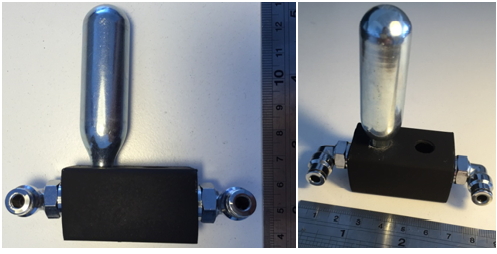
\includegraphics[scale=1]{figures/GasDetectionAgge/Prototype}
  \caption{A non working prototype of the VEGA-instrument. Here with only one cylinder added}
  \label{fig:NonProto}
\end{figure}

If the cylinders are mounted as showed in \ref{fig:NonProto} on the prototype it would be able to contain 7, since one port is used for the pressure sensor. It would be rater bulky due to the mounting of the cylinder on each side; therefore the rack system is more favorable. Overall it gives a good insight in the mechanical construction of the VEGA-instrument.

The last part not discussed is the pressure sensor, here it is possible to use an off the shelve part. Pressure sensors are today already used in harsh environments, and therefore only small modifications might be needed. A good example of a pressure sensor which is small compact and durable is the Festo SPTW-P100R-G14-VD-M12, which is a 0 to 100 bar sensor with a simple threaded connection, which simply screws into the chamber. It might be favorable with a sensor that has a range of 200 bar, but that is easily replaced if deemed necessary. A temperature sensor should also be mounted in the chamber to measure any temperature changes to make sure to get the optimal result.

With the VEGA-instrument not all the gasses specified earlier can be detected, one of the important ones is methane, but this is still a gas at the pressure between 100 and 200 bar, and can therefore not be detected with this expansion method. A way of detecting the methane would be to use a semiconductor sensor as mention in the theory section. This contains no moving parts, and is very simple to use and could be mounted inside the chamber, detecting methane when the chamber is flushed.

\subsubsection{Final physical specification}

When flying a space mission, mass, power consumption and volume of the instrument are very critical, they could be the difference flying the instrument or leaving it.

For the VEGA the configuration of it, inflects on the mass and volume, for this example the instrument carries 6 cylinders, and can therefore be reused 6 times. Dependent on the configuration of the cylinders and the camber the overall volume equates to approximately 200 $cm^3$ without the plumbing and wiring. The mass (build out of titanium) is 180 g for the cylinders, 150 g for the chamber, 120 g for sensor, 200 g for auxiliary. In all 650 g is needed for the whole instrument.

The power consumption for the instrument depends on what stage of use it is in. It does not require any power when not used. When in use the parts that use most power will be the solenoid valve for filling and emptying the chamber, which might draw a few watts when used. The gas sensor also uses a watt or less of power. In all peak consumption is assumed to be 5W, 1W when measuring, and no power use when standby.

There will also be some data processing and data transmission, but this is budgeted by the communication team. The instrument is not heavy on data, a measurement would contain between 5 and 10 Kbytes of data.

\subsection{Conclusion and further work on VEGA-instrument}

Through the design of the VEGA-instrument many different aspects has been covered, to make a comprehensive analysis of how such instrument should be designed for the harsh environment at Europa's ocean. Since this is only a theoretical instrument it is not sure that it will work at the conditions on Europa, therefore more work and test needs to be done. From the sections presented in this report, a prototype needs to be build and tests can begin, to see if it is possible to detect the gasses specified, and if other gasses also can be detected. Also an important aspect of testing is to see how large or small concentrations of a gas it is able to detect, this is dependent on the resolution of the pressure sensor and how much the gas expands when it is boiled of. The result will end up with a redesign of the instrument to accommodate the changes found under test.

Overall the instrument is a reinvention of a gas detector for high pressures, where conventional sensors are not able to work. The solution is simple and rethinks the way of sensing gas; the sensor is not perfect and is limited to a specific number of uses, due to the vacuum cylinders but this is a trade-off between complexity and simplicity. The same goes for the number of gasses it is able to detect, not all gasses can be detected but at the same time it will be able to detect more than compounds specified in this report. If the compound is liquid and mixed with the water, it could detect compounds not expected to be found and therefore the VEGA-instrument can extent it measurement range.


\section{XRF}

\autsection{HPLC}{Morten Lykke Hilligsøe}
\label{sec:hplc}
High-performance liquid chromatography (HPLC and also known as high-pressure liquid chromatography), is a chemical technique commonly used to identify, quantify and separate components of a liquid sample. Most commonly, the technique uses pressure to pump a solvent through a column filled with silica beads covered in carbohydrates. The silica beads typically have a size range of 2–50 micrometers in diameter. By mixing the sample with a polar solvent, such as acetonitrile or methanol, and passing it through the highly non-polar silica beads, each component of the sample will interact differently with the column, thereby affecting flow rates of each compound and making it possible to separate them. 

Many different HPLC techniques exist, including:
\begin{itemize}
    \item Partition chromatography
    \item Normal–phase chromatography
    \item Displacement chromatography
    \item Reversed-phase chromatography (RPC)
    \item Size-exclusion chromatography
    \item Ion-exchange chromatography
    \item Bioaffinity chromatography
    \item Aqueous normal-phase chromatography
\end{itemize}
with reversed-phase chromatography equipment being very common in chemistry and biochemistry labs all over the world. In reversed-phase chromatography, the components of the sample mixture are separated from each other based on their different interactions with the absorbent particles of the HPLC column, also known as the stationary phase. The pressurized sample/solvent mixture is referred to as a "mobile phase".

\subsubsection{Detection}
HPLC can detect a vast array of different chemical and biochemical compounds, including many compounds considered direct indicators of present life:
\begin{itemize}
    \item DNA and RNA
    \item Pharmaceuticals like aspirin, ibuprofen, or acetaminophen (Tylenol) 
    \item Salts like sodium chloride and potassium phosphate 
    \item Proteins like egg white or blood protein 
    \item Organic chemicals like polymers (e.g. polystyrene, polyethylene) 
    \item Heavy hydrocarbons like asphalt or motor oil 
    \item Many natural products such as ginseng, herbal medicines, plant extracts 
    \item Thermally unstable compounds such as trinitrotoluene (TNT) and enzymes 
\end{itemize}
HPLC will not be able detect all of these compounds using a single HPLC column, as different types of columns are optimized for different detection schemes, but a single column will still be able to detect a vast range of compounds. If more compounds are to be detected, a setup with multiple columns could also be designed. Special HPLC setups can also separate and quantify chiral enantiomers, which are considered clear indicators of life, if a set of enantiomers are found in varying concentrations. Such setups are however much less versatile, and are better suited for experiments where the examined compound is known beforehand.
Typically a marker solution is introduced to the system before the sample, in order to have some reference points. Detection limits depends very much on the optical setup (light source \& sensor) and the compound to be detected, but the separation of compounds reduces noise, thereby making it possible to detect concentrations down to µg/L, with just a few µL of sample. Because of these small sample amounts, typical column dimensions are just 2.1–4.6 mm in diameter, and 30–250 mm in length.

\subsubsection{Components}
5 major components are required for a HPLC setup:
\begin{enumerate}
    \item Pump: The pump is used to force the sample/solution mixture through the column at high pressure and at a specific flow rate. HPLC flow rates are commonly in the 0.1- to 8-mL/min range, with a pressure gradient commonly in the range of 50- to 600-bar.
    \item Injector: The injector introduces the sample into the solvent (mobile phase) flow stream at typical volumes of 5- to 20-µL. As the sample is unpressurized, the injector must be able to withstand the high pressure of the system.
    \item Column: The column’s stationary phase separates the sample components of interest using various physical and chemical parameters, such as polarity, porosity or bioaffinity. The small particles that make up the inside of the column is what causes the high pressure gradient at normal flow rates. 
    \item Detector: The detector can detect the individual compounds in the column output (elute). Usually a UV or wide spectrum light source is used in combination with a sensor which can detect individual wavelengths (e.g. photodiode array). By detecting the individual wavelength absorption of the elute, components can be distinguished, identified and quantified. The elute absorption as a function of time, is the liquid chromatogram result.
    \item Computer: Finally, a computer is used to control the HPLC instruments and might also be used to analyze the resulting chromatogram. As a result, the resulting data of each experiment can vary from megabytes when high resolution chromatographs are transferred, over kilobytes when low resolution chromatographs are transferred, and all the way down to single bytes for yes/no answers or concentrations at specific retention times. 
\end{enumerate}

Besides these components, a HPLC system usually also includes a solvent mixer and a degassing system. 
The mixer is used to create the desired mobile-phase composition, typically from a mix of water, acetonitrile and/or methanol. The mixer isn’t strictly necessary, as one can use a premade mobile-phase solution, but often a gradient of these compounds are desired throughout the experiment, as the mobility range of different compounds would otherwise be too vast, e.g. some move directly through the column, and others doesn’t move at all.

The degassing system is an essential part of any HPLC system used under normal lab conditions, as it ensures that no bubbles are created when the mobile-phase traverses the negative pressure gradient of the HPLC column. Such bubbles will ruin the experiment by blocking any further movement through the column, and can even potentially break the column.  Commonly used degassing practices for HPLC mobile phase are helium purging (removes up to 80\% of all gasses), vacuum degassing (up to 60\%) and sonication (up to 30\%). However, degassing would not be a problem on a subsea space mission for two reasons: 
\begin{enumerate}
    \item The system is closed and all solvents can easily be degassed before departure.
    \item The experiments are performed under high-pressure external conditions (below several kilometers of ice), making sure that the pressure never drops low enough for bubbles to occur.
\end{enumerate}

\subsubsection{Implementation}
To implement a HPLC system on the Europa subsea mission, the system will have to be limited in the power usage, weight, volume, and data transfer rates. The following equipment has been used as reference for calculating an approximate weight, power and volume usage:
\begin{itemize}
    \item 0.01-10mls/min, 143bar, Stainless Steel, positive displacement piston pump 
    \begin{itemize}
        \item Weight: 1.6kg
        \item Power: 40.8W
        \item Size: 139.7mm x 76.2mm x 266.7mm
    \end{itemize}
    \item Injector 
    \begin{itemize}
        \item Weight: 0.25kg
    \end{itemize}
    \item C18 Reversed-Phase HPLC Column 
    \begin{itemize}
        \item Weight: 0.2kg
        \item Size: 200mm x 2.2mm (internal)
    \end{itemize}
    \item 190-500nm, 13nm resolution, UV Detector 
    \begin{itemize}
        \item Weight: 1.5kg
        \item Power: 60W
        \item Size: 121mm x 129mm x 187mm
    \end{itemize}
    \item Solvent
    \begin{itemize}
        \item 50ml per experiment
    \end{itemize}
\end{itemize}
The chosen pump is a displacement piston pump, which are commonly used high pressure low volume applications such as HPLC systems. The possibility of using a peristaltic pump was also examined, but no peristaltic pumps were found, which could operate at +100bars of pressure. Both the injector and HPLC column weights are estimates, as no weights were given by the manufacturers. It would be nice to include a UV-Visible detector which isn’t limited to 500nm detection range, but this component was the most weight efficient solution available. Finally the solvent volume is calculated as:
\begin{equation}
    1ml/min \cdot 30min = 30ml    
\end{equation}
Which is then rounded up to 50ml per experiment, because some solvent is also necessary to flush the column before experiments.

Several connectors and peripheral equipment will also be required, resulting in a system which, during operation, requires a power input of approximately 100W, and has a total weight of around 4kg plus approximately 0.05kg of solvent per experiment. The volume of the individual components are quite large when considering the size of the penetrator, but by stripping each component down to the bare minimum, e.g. getting rid of shielding, user interfaces and AC-DC converters, the size and weight should be low enough for the HPLC solution to be contained within the penetrator. 

The data transfer rates can be calculated from the sampling frequency $f$, the sampling range $l$, the sampling resolution $\delta$, and the bit-size $b$ of each measurement point:
\begin{equation}
    f \cdot \frac{l}{\Delta} \cdot b = 1Hz \cdot \frac{500nm-190nm}{13nm} \cdot 12bits = 286bps
\end{equation}
Here the sampling frequency is chosen to be 1Hz, which is on the low end of standard sampling rates of laboratory HPLC experiments, but still good enough for most experiments. The 12 bit measurement point size gives a range from 0-4095. Since the HPLC isn’t expected to run continuously, but only run when an interesting sample has been up-concentrated, the 286bps is far below the maximum transfer limit, and both sampling frequency, sample points and bit size may be increased without creating a bottleneck.

\subsubsection{Up-concentration and injection}
The final question remains of how to get a sample up-concentrated and injected into the HPLC instrument.

\autsection{Lab-on-a-chip \& microscopic sensors}{Morten Lykke Hilligsøe}
Lab-on-a-chip (LOC) systems are a common description of microfluidic devices which can perform one or several laboratory functions on a single chip. Lab-on-a-chip systems are often characterized by a very small size in the mm2 – cm2 range, high automation requiring only sample injection and result identification, as well as zero chance of contamination due to the closed system. The small size of LOCs also results in extremely small sample sizes, sometimes reaching less than a pico liter, which can be both an advantage and a disadvantage, as small amounts of the compound of interest is necessary for detection or analysis, but the small sample volumes can be hard to handle properly. 

LOCs are typically constructed using the same lithographic techniques developed by semi-conductor industry for integrated circuit production, and consists of µm or sub-µm sized mechanical structures such as channels, mixers, valves, pumps and dosing devices, combined with micro-sensors, chemical \& biochemical reagents and/or external sensors, e.g. optical or electrical sensors. LOCs are still a novel technology, but the technology is quickly evolving and LOC solutions have found many uses, especially within biochemical and microbiological analysis, such as bacteria, virus, and bioanalyte detection.
\footnote{Ghallab, Y.; Badawy, W. (2004-01-01). "Sensing methods for dielectrophoresis phenomenon: from bulky instruments to lab-on-a-chip". IEEE Circuits and Systems Magazine 4 (3): 5–15.} \footnote{Ryan S. Pawell, David W. Inglis, Tracie J. Barber, and Robert A. Taylor, Manufacturing and wetting low-cost microfluidic cell separation devices, Biomicrofluidics 7, 056501 (2013);doi:10.1063/1.4821315} \footnote{\url{http://link.springer.com/article/10.1007/s10404-014-1464-1?sa_campaign=email/event/articleAuthor/onlineFirst}} lists advantages and disadvantages of LOCs as:

Advantages of LOCs:
\begin{itemize}
    \item low fluid volumes consumption (less waste, lower reagents costs and less required sample volumes for diagnostics)
    \item faster analysis and response times due to short diffusion distances, fast heating, high surface to volume ratios, small heat capacities.
    \item better process control because of a faster response of the system (e.g. thermal control for exothermic chemical reactions)
    \item compactness of the systems due to integration of much functionality and small volumes
    \item massive parallelization due to compactness, which allows high-throughput analysis
    \item lower fabrication costs, allowing cost-effective disposable chips, fabricated in mass production
    \item part quality may be verified automatically
    \item safer platform for chemical, radioactive or biological studies because of integration of functionality, smaller fluid volumes and stored energies
\end{itemize}
Further advantages for use on space missions, includes the possibility for complete sample processing in a single chip, e.g. filtration, lysing, mixing, chemical reactions and positioning, thereby reducing or completely dismissing any requirements for large and bulky laboratory equipment typically necessary to prepare samples before any analyte can be detected.

Disadvantages of LOCs:
\begin{itemize}
    \item novel technology and therefore not yet fully developed
    \item physical and chemical effects—like capillary forces, surface roughness, chemical interactions of construction materials on reaction processes—become more dominant on small-scale. This can sometimes make processes in LOCs more complex than in conventional lab equipment
    \item detection principles may not always scale down in a positive way, leading to low signal-to-noise ratios
    \item although the absolute geometric accuracies and precision in microfabrication are high, they are often rather poor in a relative way, compared to precision engineering for instance.
\end{itemize}
Further disadvantages for use on space missions, includes that many LOCs are single-use constructions, thereby requiring extra storage space if the experiment is to be performed multiple times, as well as mechanics to switch between chips. Then novelty of LOC technology is also exemplified in the fact, that even though the chip itself can be very small, the external equipment necessary to operate the chip is often standard laboratory equipment which hasn’t been scaled accordingly.

\subsubsection{Systems of interest}
Below is described 4 systems of interest for a life detection mission. Many other relevant projects exists, ranging from small research projects to a few readily available solutions.

\paragraph{DNA extraction and real-time PCR}
In an article from 2013, researchers at the University of North Carolina describe a “microfluidic chip integrating DNA extraction, amplification, and detection for the identification of bacteria in saliva”. Such a device could easily be used to detect if DNA is present on Europa. And because the chip has integrated filters, minimal preparation of the sample is required. The system works by filtering lysed organisms through a nanoporous aluminum oxide membrane, followed by PCR amplification of the filtered DNA in 7 parallel reaction wells. PCR amplification is the standard method of up concentrating DNA, and using this method the chip was able to detect as low as 8-12 copies of methicillin-susceptible Staphylococcus aureus DNA. PCR amplification depend primers to attach to matching DNA sequencing. For a Europa mission, any microorganisms will of course be unknown, and specific target primers will not be available. Instead a series of general primers which bind to DNA sequences common to earth life can be used to simply detect DNA. 

\paragraph{Chemical sensor}
Although more a sensor than LOC, in 2014, researchers at Vienna University of Technology have developed a very interesting sensor chip, for measuring the chemical composition of liquids. The sensor works by placing a matching set of mid-infrared quantum cascade laser and detector on a single chip connected through a 50µm waveguide. When specific molecules pass close to the waveguide, the laser light is absorbed and the molecule can be detected. The wavelength of quantum cascade lasers can be finely tuned, and lasers matching specific molecules can therefore be created, allowing for detection of various molecules, such as carbohydrates or proteins, and the small size will make it possible to have a whole array of various wavelength sensors to measure the concentration of many different compounds using a single chip.

\paragraph{Movement sensor }
A universal life detection sensor has been developed by Kasas et al. of the École Polytechnique Fédérale de Lausanne, by using a cantilever known, as known from Atomic Force Microscopy, to detect tiny fluctuations, commonly associated with the movement and metabolic activity of cells. The cantilever is essentially a metal beam which can scrape a surface, and if any living organisms get stuck on the cantilever, a laser can detect the tiny vibrations made by metabolic movement. The sensor has been successfully tested with bacteria, yeast, mouse cells, human cells, and plant cells. The unique feature of such sensor is the complete lack of knowledge required about the organism biochemistry. Where other methods rely on the assumption that extraterrestrial life has similar DNA, protein or hydrocarbon chemistry as life on earth, no such assumptions are necessary for this detection method.

\paragraph{Wet-chemical analyzers}
The National Oceanography Centre of the United Kingdom is developing chemical sensors for several of the major nutrients important for oceanic life, which includes nitrate, nitrite, ammonia, and phosphate, as well as the trace nutrients, present at low concentrations yet essential for life, such as dissolved iron and manganese, which is a tracer of hydrothermal vent emissions.  Many of these sensors are based on the principle of Flow Injection Analysis, which is commonly used in laboratory equipment, but with the goal of condensing several high precision sensors into a small device which can be used for in-situ deep ocean analysis and monitoring. Such a system is attained by use of microfluidic devices and sensors.

\subsubsection{Implementation}
Although lab-on-a-chip systems and microscopic sensors offer promising products and technologies, many of the applications which are of interest to this mission, are still in a developmental stage, and require further maturing before an extraterrestrial mission can rely on such equipment. The long life of the mission and single-use chips also hinders the effective use of such systems, and it was therefore chosen not to bring LOCs on the Europa subsea mission.

\autsection{pH \& salinity}{Kristian Sloth Lauszus and Lukas Christensen}

\autsection{Camera}{Bhaaeddin Alhomsi}

The cameras will be triggered whenever a detects a flash of light, hopefully catching a glimpse of something living. CMOS camera sensor can detect the wavelength from 350 nm (UVA) till 1100 nm (IRA), so we have to find lighting source can cover this range .
Another approach that is developing very well is that of broad band fluorescence to very deep (short wavelength) ultraviolet (UV) light. The deep UV has the advantage that at such wavelengths there is very little background fluorescence, and it is easy to identify samples containing carbon-based chemistry that could be associated with life.
Infra-red light is radiated from any object with a temperature. Even objects which are too cool to be detected optically can be studied in the infra-red.
Panoramic image (360 degree) it will give us a good understanding how is the bottom of ice shield looks like.

\subsection{Lighting}

Ambient visible light is quickly attenuated by a combination of scattering and absorption, thus requiring artificial lighting to view items underwater with any degree of clarity. We see things in color because objects reflect wavelengths of light that represent the colors of the visible spectrum. Artificial lighting is therefore necessary near the illuminated object to view it in true color with intensity. Underwater lamps provide this capability.
Lamps convert electrical energy into light. The main types or classes of artificial lamps/light sources used in underwater lighting are incandescent, fluorescent, high intensity gas discharge, and light-emitting diode (LED) - each with its strengths and weaknesses. All types of light are meant to augment the natural light present in the environment.
 The flash lamps provide a short duration (about 0.005 see) heat pulse. The short burst of energy results in a momentary rise in the surface temperature of the part. The temperature rise may be detrimental to the top layer of the part being exposed. Therefore, it is necessary to ensure the non-destructive nature of the technique. Amount of the temperature rise determines whether the flash-lamp heating would be detrimental to the part. 
the flash duration is about 0.005 sec. Because of the short flash duration, relatively little amount of heat is imparted. The part temperature on the surface rises until end of the flash duration and then drops quickly due to the heat radiation and convection from the surface and the heat conduction into the part. The temperature rise on the part surface can be high enough to damage the top layer of the part.
The table below, shows the major types of artificial lighting systems, as well as their respective characteristics.
\begin{figure}[htb]
\centering
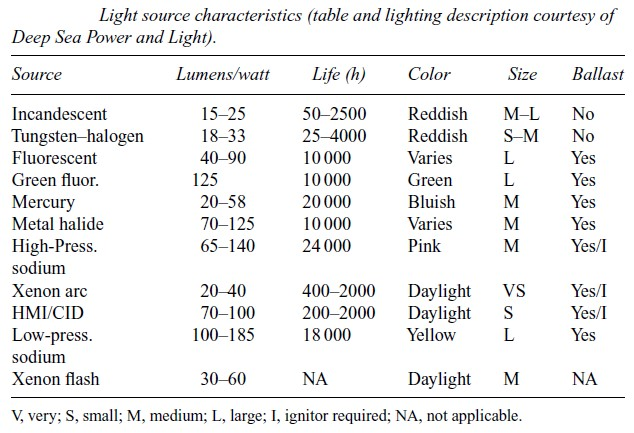
\includegraphics[scale=0.75]{figures/camera/bh6.jpg}
\caption{Light source characteristics}
\end{figure}
\\
Incandescent – The incandescent lamp was the first artificial light bulb invented.
Electricity is passed through a thin metal element, heating it to a high enough temperature to glow (thus producing light). It is inefficient as a lighting source with approximately 90 \% of the energy wasted as heat. Halogen bulbs are an improved incandescent. Light energy output is about 15 \% of energy input,  instead of 10 \%, allowing them to produce about 50 \% more light from the same amount of electrical power. However, the halogen bulb capsule is under high pressure instead of a vacuum or low-pressure noble gas (as with regular
incandescent lamps) and, although much smaller, its hotter filament temperature causes the bulbs to have a very hot surface. This means that such glass bulbs can explode if broken, or if operated with residue (such as fingerprints) on them. The risk of burns or fire is also greater than other bulbs, leading to their prohibition in
some underwater applications. Halogen capsules can be put inside regular bulbs or dichroic reflectors, either for aesthetics or for safety. Good halogen bulbs produce a sunshine-like white light, while regular incandescent bulbs produce a light between sunlight and candlelight.

\begin{figure}[htb]
\centering
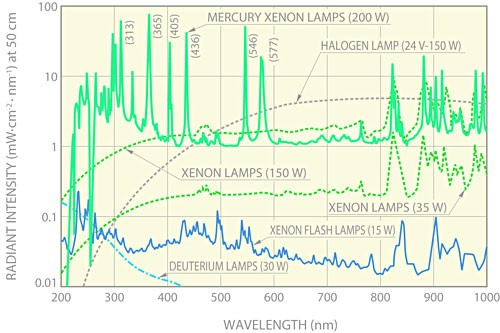
\includegraphics[scale=1]{figures/camera/bh7.jpg}
\caption{Lamp wavelength}
\end{figure}

A fluorescent lamp is a type of lamp that uses electricity to excite
mercury vapour in argon or neon gas, producing short-wave ultraviolet light. This light then causes a phosphor coating on the light tube to fluoresce, producing visible light. Fluorescent bulbs are about 40 \% efficient, meaning that for the same amount of light they use one-fourth the power and produce one-sixth the heat of a regular incandescent. Fluorescents typically do not have the luminescent output capacity per unit volume of other types of lighting, making them (in many underwater applications) a poor choice for underwater artificial light sources.

High-intensity discharge – High-intensity discharge (HID) lamps include the
following types of electrical lights: Mercury vapour, metal halide, high pressure sodium and, less common, xenon short-arc lamps. The light-producing element of these lamp types is a well-stabilized arc discharge contained within a refractory envelope (arc tube) with wall loading (power intensity per unit area of the arc tube) in excess of 3W/cm2 (19.4 W/in2). Compared to fluorescent and incandescent lamps, HID lamps produce a large quantity of light in a small package, making them well suited for mounting on underwater vehicles. The most common HID lights used in underwater work are of the metal halide type.

LED – A light-emitting diode (LED) is a semiconductor device that emits incoherent narrow-spectrum light when electrically biased in the forward direction. This effect is a form of electroluminescence. The color of the emitted light depends on the chemical composition of the semiconducting material used, and can be near-ultraviolet, visible, or infra-red. LED technology is useful for underwater lighting because of its low power consumption, low heat generation, instantaneous on/off control, continuity of color throughout the life of the diode, extremely long life, and relatively low cost of manufacture. LED lighting is a rapidly evolving technology \cite{lighting}.

We will select xenon lamp 150 W, because it will provide us with good radiant intensity for the whole wavelength range.

\subsection{Reflector}
An efficient reflector will not only maximize the light output that falls on the target, but will also direct heat forward and away from the lamp. The shape of the reflector will be the main determinant in how the light output is directed. Most are parabolic, but ellipsoidal reflectors are often used in underwater applications to focus light through a small opening in a pressure housing. 

The surface condition of a reflector
will determine how the light output will be dispersed and diffused. The majority of reflectors are made of pure, highly polished aluminium that will reflect light back at roughly the same angle to the normal at which it was incident. By adding dimples or peens to the surface, the reflected light is dispersed or spread out. When a plain white surface is used, the reflected light is diffused in all directions.

\subsection{The wavelength range of optical radiation}

The term "optical radiation" refers to electromagnetic radiation in the wavelength range between 100 nm and 1 mm. The terms "light" and "visible radiation" (VIS) refer to the wavelength range between 400 nm and 800 nm, which can be perceived by the human eye. Optical radiation with wavelengths shorter than 400 nm is called ultraviolet (UV) radiation and is further subdivided in UV-A, UV-B and UV-C ranges. Similarly, infra-red (IR) radiation covers the wavelength range above 800 nm and is subdivided in IR-A, IR-B and IR-C ranges.

\begin{figure}[htb]
\centering
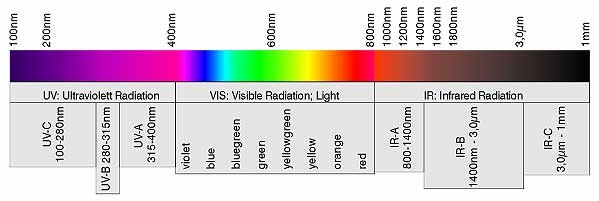
\includegraphics[scale=1]{figures/camera/bh8.jpg}
\caption{The wavelength range of optical radiation}
\end{figure}

The sensitivity of the human eye to light of a certain intensity varies strongly over the wavelength range between 380 and 800 nm. Under daylight conditions, the average normal sighted human eye is most sensitive at a wavelength of 555 nm.

\subsection{Camera}

The ECAM imaging system delivers cost-effective, short lead-time, high-performance, and reliable space imaging as a modular off-the-shelf solution. The C50 utilizes a CMOS image sensor with integral RGB Bayer Pattern color filter array. The sensor outputs 10-bit pixels that are square-root companded to 8-bits before being transmitted to the DVR on a 200 Mbit/s serial link.. Preprocessing typically includes Bayer Pattern interpolation and direct conversion to the YCbCr color space using a 5 x 5 filter kernel. The video is also reformatted as needed for input to either a JPEG (lossy) or Huffman First Difference (lossless) compressor. The C50 is highly configurable. The exposure and gain may be adjusted to support widely varying scene. The optical lens made of a material that has substantially the same index of refraction as that of water.$http://www.msss.com/brochures/c50.pdf$

\begin{figure}[htb]
\centering
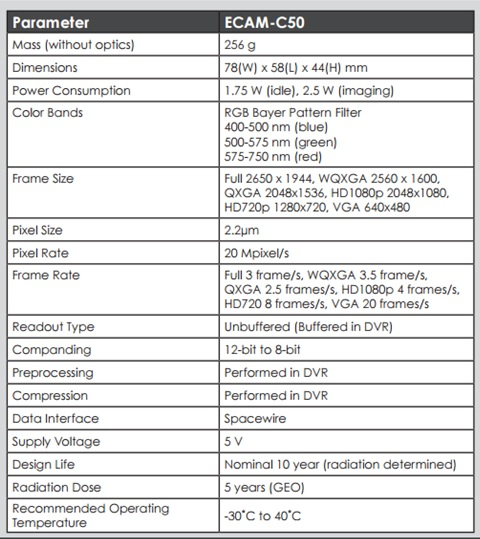
\includegraphics[width=.48\textwidth]{figures/camera/bh10.jpg}
\caption{Camera parameters}
\end{figure}

CMOS sensor can detect the wavelength from 350 nm (UVA) till 1100 nm (IRA), so we have to find lighting source can cover this range .

\begin{figure}[htb]
\centering
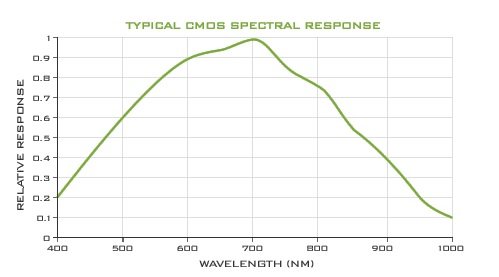
\includegraphics[scale=1]{figures/camera/bh9.jpg}
\caption{CMOS spectral response}
\end{figure}

\subsection{Panoramic Images}

To take a panorama, the camera is rotated at fixed angular increments, taking an image at each point. These images can then be assembled (stitched) using stitching software, which allows the images to be aligned and combined into a single seamless panoramic image, either automatically (using image analysis) or manually (with user supplied control points).For this mission we will fix the camera on the robotic arm, and the arm will rotate and taking images. These images will sent to the earth. In the earth, the images aligned and combined into panoramic image.
The rotation angle depend on camera field of view , in or proposed camera the field of view angle is approximately 70 degree , so to build 360 panoramic image we need 5 photos with rotation angle 70 degree between each shoot.


\section{Microscope}
